% Project Management Plan Documentation Template %
% Template made following ISO/IEC/IEEE 16326:2009 %

% Author : Alejandro Muñoz Del Álamo %
% Copyright 2019 %

% Project Overview File %


\part{Prolegómeno}

\chapter{Introducción}
\thispagestyle{chapterpage}

\section{Motivación}
El sector de los juegos de rol está creciendo a pasos 
agigantados. Hoy en día existe un extensísimo 
catálogo de juegos de rol, que varían en función de la 
ambientación del ``universo'' en el que nos sumergimos. Por 
ejemplo, \textit{Dragones y Mazmorras} utiliza una 
ambientación medieval con elementos fantásticos, tales como 
magia y dragones, mientras que \textit{Warhammer 40.000} 
está basado en un futuro distópico en el que se mezclan 
elementos de ciencia ficción con elementos de fantasía 
heroica. \medskip

Debido a la expansión de este sector, y gracias al avance 
de la tecnología, podemos encontrar un sinfín de aplicaciones 
que tratan de mejorar la experiencia de los jugadores, 
desde juegos de mesa que hacen uso de sistemas de 
reproducción (\textit{CD}, \textit{DVD}, 
\textit{Blu-Ray}) para hacer del juego una experiencia 
interactiva (\textit{Atmosfear}, \textit{Piratas
del Caribe: El Cofre del Hombre Muerto}, \textit{Trivial 
Pursuit}, \textit{Cluedo}), hasta juegos de rol completamente
virtualizados que nos permiten sumergirnos en ellos, contemplar
sus parajes, disfrutar de su ambientación, y en algunos casos, 
nos permiten participar con jugadores de cualquier parte del 
mundo a través de la red (\textit{World of Warcraft}, \textit{Diablo III}, 
\textit{Black Desert Online}). \medskip

Dentro de este amplio espectro de posibilidades, los juegos de rol 
tradicionales también disponen de aplicaciones que enriquecen el 
transcurso de las partidas, y que proveen prestaciones útiles para las 
mismas, como lanzadores de dados virtuales, generadores de mazmorras, 
contadores de iniciativa, compendios de habilidades, etc. \medskip

Entre todas las utilidades que encontramos, cabe destacar las aplicaciones 
conocidas como \textit{generadores de personaje}. Estas facilitan a los 
jugadores todo lo necesario para desarrollar rápidamente la información 
indispensable de un personaje para poder interpretarlo en una partida. \medskip

Por otro lado, puesto que la tecnología tiene un ritmo de avance trepidante, 
y más aún la informática, hoy en día podemos echar cuenta de servicios 
que simplifican tareas cuya ejecución resultaba impensable en el pasado.
\medskip

Uno de estos servicios es la Web Semántica, que se basa en la idea de 
describir el contenido, el significado y la relación 
de los datos, de manera que sea posible evaluarlos automáticamente por 
máquinas de procesamiento, como pueden ser los ordenadores o los 
\textit{smartphones}.
\medskip

El planteamiento del presente proyecto surge de la concepción de una 
aplicación informática destinada a ampliar las funcionalidades de 
los generadores de personaje, innovando en el desarrollo de la misma 
al aplicar tecnologías de Web Semántica.\medskip


\section{Alcance}
El alcance de este proyecto comprende el desarrollo de una 
aplicación móvil para generar perfiles de personajes que 
puedan formar parte de una partida o campaña de un juego 
de rol, cuya base de datos esté incluida en la aplicación. \medskip

No forma parte del alcance de este proyecto el desarrollo 
de la base de datos del juego de rol, aunque ha sido 
necesario para poder realizar la sección de pruebas del
proyecto.

\section{Objetivos}
El sistema va a tener tres finalidades claramente diferenciadas:
\begin{itemize}

    \item \textbf{Selección de juego}:La aplicación podrá dar 
    acceso a varios juegos, de manera que se pueda alternar 
    entre éstos, permitiendo utilizar el mismo mecanismo para 
    el catálogo de juegos disponible.

    \item \textbf{Creación/Modificación de personaje}: La 
    aplicación permitirá al usuario seleccionar la información
    necesaria para la creación de un personaje a su gusto 
    mediante un proceso guiado paso a paso. En caso de que el 
    personaje ya exista, permitirá al usuario visualizar y realizar 
    modificaciones a la información mostrada.

    \item \textbf{Automatización del proceso de cálculo 
    de habilidades}: La aplicación facilitará al usuario una 
    interfaz en la que, al indicar la habilidad que desea 
    utilizar, y el resultado de su lanzamiento de dados, se 
    devuelva el resultado total que se debe aplicar en el 
    combate. También podrá calcular el resultado de tiradas 
    enfrentadas.

\end{itemize}

Además, la aplicación deberá hacer muestra de las siguientes 
cualidades: 
\begin{itemize}

    \item \textbf{Generalidad}: La aplicación no estará directamente 
    vinculada a la información específica de un juego, de forma que 
    sea posible procesar diferentes bancos de datos, y por tanto, 
    se pueda utilizar la misma aplicación para varias versiones 
    distintas del mismo juego, o incluso para juegos completamente 
    diferentes.

    \item \textbf{Sencillez}: La aplicación dispondrá de una interfaz 
    simple y agradable, que permita al usuario hacer uso de sus 
    funciones de forma asequible, sea cual fuere la complejidad del 
    juego seleccionado.

\end{itemize}


% Plantilla Tabla Requisitos Funcionales
%\begin{changemargin}{-1cm}{-1cm}
%    \begin{table}[h] 
%        \centering
%        \begin{tabular}{|l|m{10cm}|}
%            \hline
%            [Código objetivo] & [Nombre Objetivo] \\ 
%            \hline
%            \hline
%            Descripción & [Descripción Objetivo] \\
%            \hline
%            Comentarios & [Comentarios Objetivo] \\
%            \hline
%        \end{tabular}
%        \caption{Objetivo [Nº]. [\textit{Nombre Objetivo}]}
%    \end{table}
%\end{changemargin}

\section{Glosario de Términos}
\begin{itemize}

    % Añadir WebSemántica

    \item \textbf{\textit{Android}}: Sistema operativo que se emplea 
    en dispositivos móviles, por lo general con pantalla táctil. 
    De este modo, es posible encontrar tabletas, teléfonos móviles 
    y relojes equipados con Android, aunque el software también 
    se usa en otros dispositivos. 
    % https://definicion.de/android/ 

    \item \textbf{\textit{Blazegraph}}: Base de datos de grafos de 
    código abierto, escalable y de alto rendimiento basada en 
    estándares. Escrito completamente en \emph{Java}, la plataforma soporta 
    las familias de especificaciones \emph{Blueprint} y \textbf{RDF}/\textbf{SPARQL 1.1}
    incluyendo consultas, actualizaciones, consultas federadas básicas
    y descripción de servicios. 
    % https://wiki.blazegraph.com/wiki/index.php/About_Blazegraph
    
    \item \textbf{\textit{C\#}}: Lenguaje de programación multiparadigma 
    desarrollado y estandarizado por Microsoft como parte de su 
    plataforma \textbf{\net}, que después fue aprobado como un estándar por la
    ECMA (\emph{ECMA-334}) e ISO (\emph{ISO/IEC 23270}). 
    C\# es uno de los lenguajes de programación diseñados para la 
    infraestructura de lenguaje común. Su sintaxis básica deriva de 
    \emph{C/C++} y utiliza el modelo de objetos de la plataforma \\net, 
    similar al de \emph{Java}, aunque incluye mejoras derivadas de otros lenguajes.
    % https://es.wikipedia.org/wiki/C_Sharp


    \item \textbf{\textit{RDFSharp}}: \emph{Framework} de código 
    abierto \textbf{C\#} diseñado para facilitar la creación de 
    aplicaciones \emph{\net} basadas en el modelo \textbf{RDF}, 
    que representa una solución didáctica directa para comenzar 
    a trabajar con conceptos de \emph{Semántica Web}.
    % https://www.w3.org/2001/sw/wiki/RDFSharp

    \item \textbf{\textit{Git}}: Software de control de versiones 
    diseñado por \emph{Linus Torvalds}, pensando en la eficiencia 
    y la confiabilidad del mantenimiento de versiones de aplicaciones 
    cuando éstas tienen un gran número de archivos de código fuente. 
    Su propósito es llevar registro de los cambios en archivos de 
    computadora y coordinar el trabajo que varias personas realizan 
    sobre archivos compartidos.
    % https://es.wikipedia.org/wiki/Git

    \item \textbf{\textit{GitHub}}: GitHub es una plataforma de desarrollo 
    colaborativo de software para alojar proyectos utilizando el sistema de 
    control de versiones \textbf{Git}.
    % https://conociendogithub.readthedocs.io/en/latest/data/introduccion/

    \item \textbf{\textit{IDE}}: \emph{(Integrated Development Environment)} 
    Aplicación con numerosas características que se pueden usar para muchos 
    aspectos del desarrollo de software.
    %  https://docs.microsoft.com/es-es/visualstudio/get-started/visual-studio-ide?view=vs-2019

    \item \textbf{\textit{iOS}}: Sistema operativo móvil de la multinacional
    \emph{Apple Inc}. Originalmente desarrollado para el iPhone (iPhone OS), 
    después se ha usado en dispositivos como el iPod touch y el iPad. 
    No permite su instalación en hardware de terceros.
    % https://es.wikipedia.org/wiki/IOS
    
    \item \textbf{\textit{Metodología Ágil}}: Las metodologías ágiles son 
    métodos de desarrollo de software en los que las necesidades y soluciones 
    evolucionan a través de una colaboración estrecha entre equipos 
    multidisciplinarios. Se caracterizan por enfatizar la comunicación 
    frente a la documentación, por el desarrollo evolutivo y por su 
    flexibilidad.
    % https://es.wikiversity.org/wiki/Metodolog%C3%ADas_%C3%A1giles_de_desarrollo_software
    
    \item \textbf{\textit{Modelo}}: Las clases de modelo son clases no 
    visuales que encapsulan los datos de la aplicación. Por lo tanto, se 
    puede considerar que el modelo representa el modelo de dominio de la 
    aplicación, que normalmente incluye un modelo de datos junto con la 
    lógica de validación y negocios. 
    % https://docs.microsoft.com/es-es/xamarin/xamarin-forms/enterprise-application-patterns/mvvm

    \item \textbf{\textit{Modelo de Vista}}: El modelo de vista implementa las 
    propiedades y los comandos a los que la vista puede enlazarse y notifica 
    a la vista de cualquier cambio de estado a través de los eventos de 
    notificación de cambios. Las propiedades y los comandos que proporciona 
    el modelo de vista definen la funcionalidad que ofrece la interfaz de 
    usuario, pero la vista determina cómo se mostrará esa funcionalidad.
    % https://docs.microsoft.com/es-es/xamarin/xamarin-forms/enterprise-application-patterns/mvvm
    
    \item \textbf{\textit{MVVM}}: Patrón de arquitectura de software que
    ayuda a separar la lógica de negocios y presentación de una aplicación 
    de su interfaz de usuario. 
    % https://docs.microsoft.com/es-es/xamarin/xamarin-forms/enterprise-application-patterns/mvvm

    \item \textbf{\textit{Ontología}}:  Definición formal de tipos, propiedades, 
    y relaciones entre entidades que realmente o fundamentalmente existen 
    para un dominio de discusión en particular. Es una aplicación práctica 
    de la ontología filosófica, con una taxonomía.
    %  https://es.wikipedia.org/wiki/Ontolog%C3%ADa_(inform%C3%A1tica)

    \item \textbf{\textit{OWL}}: \emph{(Ontology Web Language)} es un lenguaje 
    de marcado semántico para publicar y compartir ontologías en la 
    World Wide Web. OWL se desarrolla como una extensión de vocabulario 
    de \textbf{RDF} y es derivado del lenguaje DAML + OIL asi.
    % https://www.w3.org/TR/owl-ref/


    \item \textbf{\textit{Protégé}}: Framework editor de ontologías de 
    código abierto y gratuito para construir sistemas inteligentes.
    % https://protege.stanford.edu/

    \item \textbf{\textit{RDF}}: \emph{(Resource Description Framework)} 
    Modelo estándar para el intercambio de datos en la Web. RDF 
    tiene características que facilitan la fusión de datos incluso si 
    los esquemas subyacentes difieren, y admite específicamente la 
    evolución de los esquemas a lo largo del tiempo sin requerir que 
    se cambien todos los consumidores de datos.
    % https://www.w3.org/RDF/

    \item \textbf{\textit{RDFS}}: \emph{RDF Schema} es una 
    extensión del vocabulario básico de \emph{RDF} que proporciona un 
    vocabulario de modelado de datos para los datos relativos a este modelo.
    % https://www.w3.org/TR/rdf-schema/

    \item \textbf{\textit{Scrum}}: Marco de trabajo para la gestión y 
    desarrollo del software basada en un proceso iterativo e incremental 
    utilizado comúnmente en entornos basados en el desarrollo ágil del
    software.
    % Carmen Lasa Gómez Alonso Alvarez García, Rafael de las Heras del Dedo. 
    % "Métodos Ágiles y Scrum". Anaya Multimedia, 2012.
    
    \item \textbf{\textit{SonarQube}}: Herramienta de revisión automática 
    de código para detectar errores, vulnerabilidades y olores de código 
    en su código. Se puede integrar con su flujo de trabajo existente 
    para permitir la inspección continua de código en todas las ramas 
    de su proyecto y solicitudes de extracción.
    % https://docs.sonarqube.org/latest/

    \item \textbf{\textit{SPARQL}}: \emph{(SPARQL Protocol and RDF Query 
    Language)} es un lenguaje y protocolo de consulta para \emph{RDF}. 
    % https://www.w3.org/TR/rdf-sparql-protocol/

    \item \textbf{\textit{Sprint}}: Período en el cual se lleva el 
    desarrollo de una tarea.
    % Carmen Lasa Gómez Alonso Alvarez García, Rafael de las Heras del Dedo. 
    % "Métodos Ágiles y Scrum". Anaya Multimedia, 2012.

    \item \textbf{\textit{Tarsier}}: Herramienta para la visualización 
    interactiva en 3D de grafos RDF.\@
    % Fabio Viola, Luca Roffia, Francesco Antoniazzi, Alfredo D’Elia, Cristiano Aguzzi and Tullio Salmon Cinotti     
    % "Interactive 3D Exploration of RDF Graphs through Semantic Planes" 17 August 2018

    \item \textbf{\textit{UML}}: \emph{(Unified Modeling Language)} es el 
    lenguaje de modelado de sistemas de software más conocido y utilizado 
    en la actualidad.
    % https://es.wikipedia.org/wiki/Lenguaje_unificado_de_modelado

    \item \textbf{\textit{Vista}}: La vista es responsable de definir 
    la estructura, el diseño y la apariencia de lo que el usuario ve 
    en la pantalla. Idealmente, cada vista se define en XAML, con un 
    código subyacente limitado que no contiene la lógica de negocios. 
    Sin embargo, en algunos casos, el código subyacente podría contener 
    lógica de la interfaz de usuario que implementa el comportamiento 
    visual que es difícil de expresar en XAML, como animaciones.
    % https://docs.microsoft.com/es-es/xamarin/xamarin-forms/enterprise-application-patterns/mvvm

    \item \textbf{\textit{Visual Studio}}: El \emph{IDE} de Visual Studio 
    es un panel de inicio creativo que se puede usar para editar, 
    depurar y compilar código y, después, publicar una aplicación.
    Más allá del editor estándar y el depurador que proporcionan la 
    mayoría de \emph{IDE}, Visual Studio incluye compiladores, herramientas 
    de finalización de código, diseñadores gráficos y muchas más 
    características para facilitar el proceso de desarrollo de software.
    % https://docs.microsoft.com/es-es/visualstudio/get-started/visual-studio-ide?view=vs-2019

    \item \textbf{\textit{W3C}}: \emph{(World Wide Web Consortium)} Consorcio 
    internacional que produce recomendaciones para la \emph{WWW}.
    % https://www.w3c.es/Consorcio/

    \item \textbf{\textit{WWW}}: \emph{(World Wide Web)} Sistema de distribución 
    de información basado en hipertexto o hipermedios enlazados y accesibles 
    a través de Internet. 
    % https://es.wikipedia.org/wiki/World_Wide_Web

    \item \textbf{\textit{Xamarin}}: Xamarin es una plataforma de código 
    abierto para compilar aplicaciones modernas y de rendimiento para iOS, 
    Android y Windows con \net.
    % https://docs.microsoft.com/es-es/xamarin/get-started/what-is-xamarin

    \item \textbf{\textit{Xamarin.Forms}}: Xamarin.Forms es un marco de 
    interfaz de usuario de código abierto. Xamarin.Forms permite a los 
    desarrolladores compilar aplicaciones de Android, iOS y Windows 
    desde un único código base compartido.
    % https://docs.microsoft.com/es-es/xamarin/get-started/what-is-xamarin-forms

    \item \textbf{\textit{XAML}}: \emph{(eXtensible Application Markup 
    Language)} Lenguaje basado en XML creado por \emph{Microsoft} como una 
    alternativa a código de programación para la creación de instancias 
    e inicialización de objetos, y la organización de esos objetos en 
    jerarquías de elementos primarios y secundarios.
    % https://docs.microsoft.com/es-es/xamarin/xamarin-forms/xaml/xaml-basics/

    \item \textbf{\textit{Web Semántica}}: ``\textit{Extensión de la actual 
    web en la que a la información disponible se le otorga un significado 
    bien definido que permita a los ordenadores y las personas trabajar en 
    cooperación. Se basa en la idea de tener datos en la web definidos y 
    vinculados de modo que puedan usarse para un descubrimiento, 
    automatización y reutilización entre varias aplicaciones.}''
    % Hendler, James, Berners-Lee, Tim and Miller, Eric 
    %"Integrating Applications on the Semantic Web," 
    % Journal of the Institute of Electrical Engineers of Japan, 
    % Vol 122(10), October, 2002, p. 676-680.


\end{itemize}

\section{Metodología}
\subsection{Metodologías de desarrollo software}
El desarrollo de software está en constante cambio. 
Esto se debe en parte a la continua aparición de nuevas tecnologías que 
transforman los modelos teóricos vigentes. Por otro lado, existe una 
barrera entre las herramientas de desarrollo y la metodología que impide 
la puesta en práctica de muchos de los modelos propuestos. No es fácil 
adaptarse de manera adecuada a una metodología de desarrollo de software, 
lo que resulta en un proceso con posibles demoras. No obstante, \textit{el uso de una metodología adecuada ha probado ser un pilar para 
el desarrolllo de un proyecto de construcción de software} (Moyo, Fonde, Soganile, Dzawo \& Madzima, 2013). \medskip


%Moyo, B., Gonde, P., Soganile, N., Dzawo, G., & Madzima, K.
%(2013). Empirical evaluation of software development
%methodology selection consistency: A case study using
%Analytical Hierarchy Process. Proceedings of the International Conference on Software Engineering Research
%and Practice (SERP), (págs. 1-7). Athens.

De aquí es posible extraer dos ideas claras: la primera es que adaptarse a una metodología es una tarea complicada, 
pero que de lograrse con éxito, son claros los beneficios obtenidos frente a los resultados si no se hubiera 
realizado dicha adaptación. La segunda es que resulta necesario realizar un estudio para conocer 
cuáles son las métodologías existentes, cuáles están presentes en el mercado, conocer sus ventajas e inconvenientes, 
conocer su proceso de implementación y conocer si su alcance está alineado con el objetivo que se desea lograr. \medskip

Actualmente existe un gran abanico de metodologías, las cuales se adaptan en mayor o menor medida al tipo de producto 
que se pretende desarrollar. La gran mayoría de ellas están basadas en alguno de los siguientes modelos de desarrollo 
de software:
\begin{itemize}
    \item \textbf{Desarrollo en cascada}: \textit{Enfoque metodológico que ordena rigurosamente las etapas de proceso para el 
    desarrollo de software, de forma que el inicio de cada etapa debe esperar a la finalización de la etapa 
    anterior} (Pressman, 1995). 

    %Pressman, R. (1995). Ingeniería del Software: Un enfoque práctico, (3ª Edición, Pag. 26-30).México,MCGraw Hill.
    De acuerdo a Winston Royce, que propuso dicho modelo, los beneficios de esta metodología surgen cuando no existen 
    fechas inmediatas de implementación, de manera que se dispone del tiempo apropiado para desarrollar cada fase.
    Cabe destacar que para que este modelo tenga un indice de riesgo bajo, los requerimientos deben ser claros y deben 
    haberse establecido oficialmente en la primera parte del proyecto.

    \begin{figure}[H]
        \centering
        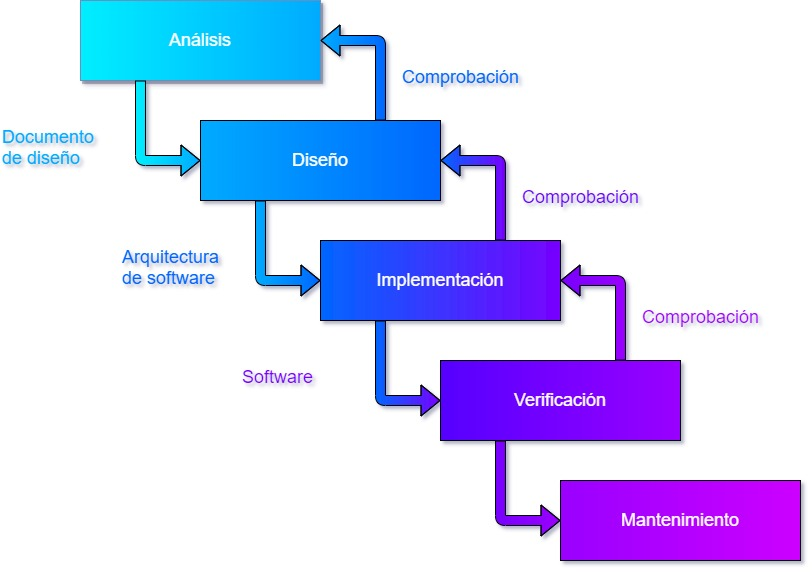
\includegraphics[width=5cm]{Figures/modelo_cascada.jpg}
        \caption{Modelo de desarrollo en cascada}
    \end{figure}
    \newpage

    \item \textbf{Desarrollo en espiral}: Este modelo, presentado por Barry Boehm, permite analizar con mayor profundidad 
    las etapas comprendidas en el desarrollo de un producto software. Las actividades de este modelo se conforman en una espiral, 
    en la que cada bucle o iteración representa un conjunto de actividades. Las actividades no están fijadas a ninguna prioridad, 
    sino que las siguientes se eligen en función del análisis de riesgo, comenzando por el bucle interior.

    \begin{figure}[H]
        \centering
        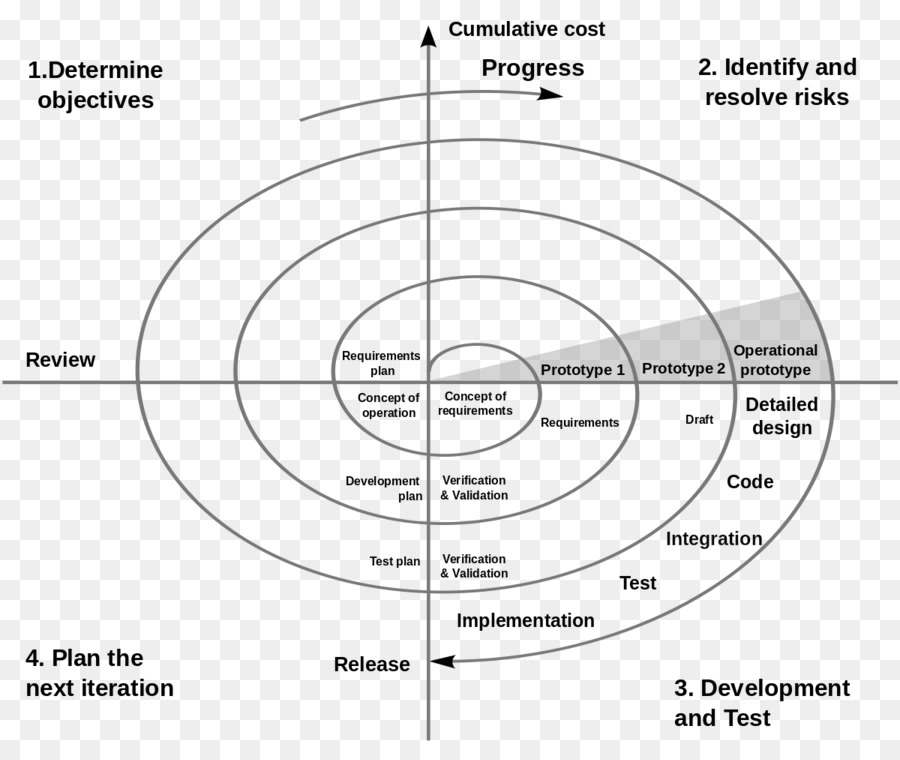
\includegraphics[width=5cm]{Figures/modelo_espiral.jpg}
        \caption{Modelo de desarrollo en espiral}
    \end{figure}

    \item \textbf{Desarrollo con prototipos}: \textit{El desarrollo de software basado en prototipos promueve la comunicación entre el cliente
    y el equipo de programadoroes, a la vez que logra una rápida integración de cambios y acorta el tiempo de desarrollo del proyecto.}
    (Ventura, Salinas, Álamos y Arreola, 2015). El paradigma de desarrollo basado en prototipos consiste en un proceso iterativo que tiene cinco 
    fases:
    % RAMÓN VENTURA ROQUE HERNÁNDEZ, JUAN MANUEL SALINAS ESCANDÓN, CALEB ALFREDO ÁLAMOS ACOSTA, ROBERTO ARREOLA RIVERA
    %Comparación empírica entre el proceso unificado y el desarrollo de software por prototipos. 
    \begin{enumerate}
        \item \textbf{\textit{Comunicación}}: Se indica un conjunto de objetivos que el software debe cumplir.
        \item \textbf{\textit{Plan rápido}}: Se propone una estrategia para llevar a cabo el desarrollo
        \item \textbf{\textit{Diseño rápido}}: Se realiza el diseño de una interfaz gráfica rápidamente.
        \item \textbf{\textit{Construcción}}: Se construye el prototipo del sistema software.
        \item \textbf{\textit{Entrega y retroalimentación}}: Se ebtrega el prototipo y el cliente realiza una 
        retroalimentación al equipo, que da inicio a una nueva iteración que incorpora los ajustes indicados en la 
        información dada por el cliente.
    \end{enumerate}
    
    \begin{figure}[H]
        \centering
        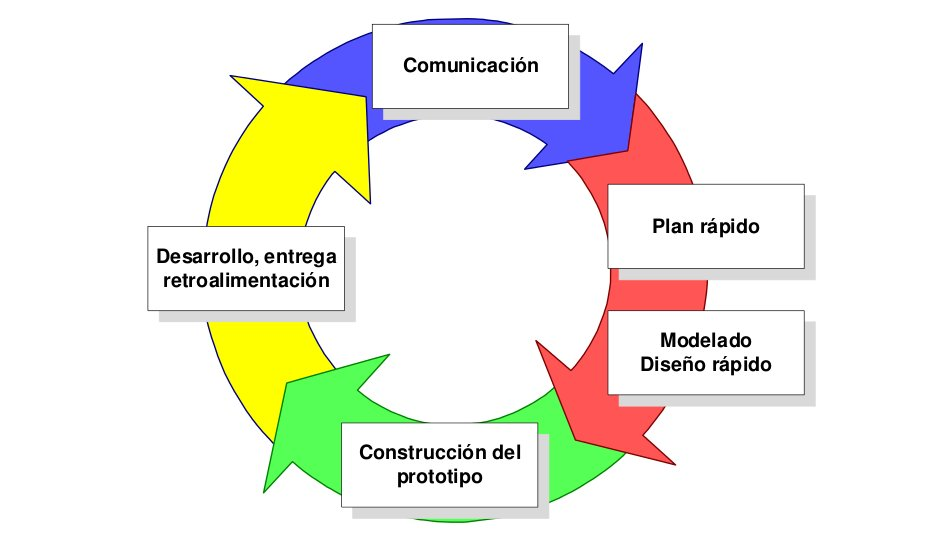
\includegraphics[width=5cm]{Figures/modelo_prototipos.jpeg}
        \caption{Modelo de desarrollo con prototipos}
    \end{figure}

    \item \textbf{Desarrollo incremental}:Consiste en un modelo iterativo que cuenta con una serie de fases de desarrollo
    (Análisis, Diseño, Implementación, Pruebas) que se repiten en orden de manera que cada vez que se finaliza una iteración, 
    el producto está mas refinado, siendo el objetivo llegar al producto final.

    \begin{figure}[H]
        \centering
        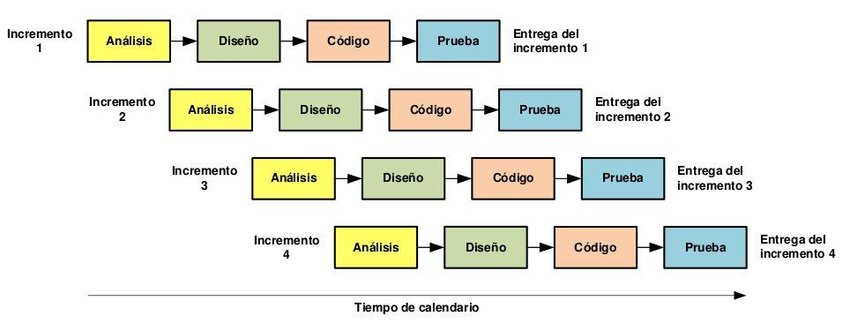
\includegraphics[width=8cm]{Figures/modelo_incremental.png}
        \caption{Modelo de desarrollo incremental}
    \end{figure}
\end{itemize}

\subsection{Metodologías Ágiles}
En febrero de 2001 nace el término \textbf{ágil} aplicado al desarrollo de software, tras una reunión celebrada en 
\textit{Utah (EEUU)}. El objetivo de la misma fue esbozar valores y principios que deberían permitir desarrollar 
software de manera rápida, dando respuesta a los cambios surgidos durante el desarrollo del proyecto. Se pretende 
con esto ofrecer alternativas a los procesos de desarollo software tradicionales, rígidos y dirigidos por la documentación 
que se generaba en cada una de las etapas del proceso.\medskip

El punto de partida para ello fue el \textbf{Manifiesto Ágil}: %agilemanifesto.org
documento que resume la filosofía ágil, en el cual se valoran los siguientes elementos:
\begin{itemize}
    \item \textbf{El individuo y las interacciones del equipo de desarrollo sobre el proceso y las herramientas}:
    Las personas que forman parte del proyecto son el principal factor de éxito de un proyecto, de manera que el entorno
    influye menos que la bondad del equipo que realiza el desarrollo. Es preferible que el entorno se adapte al equipo.

    \item \textbf{Desarrollo de software útil es mejor que conseguir una buena documentación}:
    La regla a seguir es \textit{producir sólo documentos que sean necesarios inmediatamente para tomar una 
    decisión importante}.

    \item \textbf{La colaboración del cliente sobre la negociación de un contrato}: Se propone una interacción 
    constante entre cliente y desarrolladores, de manera que esta colaboración permita marcar el ritmo del 
    proyecto y asegure el éxito del mismo.

    \item \textbf{Respuesta rápida a los cambios es mejor que seguir un plan de forma estricta}:
    La habilidad de responder a los cambios determina el éxito o fracaso del proyecto, de manera que lo
    más importante de la planificación es su flexibilidad.
\end{itemize} 

Los principios del \textit{Manifiesto Ágil} se basan en estos valores, que a su vez hacen de fundamentos de 
todas las metodologías ágiles, orientando el desarrollo a la rápida obtención de un producto funcional 
aunque no tenga todas sus funciones implementadas. \medskip

Del modelo de desarrollo ágil se pueden encontrar diversas metodologías, como \textbf{eXtreme Programming} (Stephens \& Rosenberg, 2003),
\textbf{Scrum} (Sutherland \& Schwaber, 2010) o \textbf{Crystal Clear} (Cockburn, 2004). 
Para este proyecto se ha tomado la decisión de seguir la metodología \textit{\textbf{Scrum}} ya que debido a la naturaleza y complejidad del mismo, 
es posible que sea necesario realizar cambios en el planteamiento del proyecto durante el proceso de desarrollo. \medskip

\subsection{SCRUM}
\begin{figure}[H]
    \centering
    
\includegraphics[width=5cm]{Images/Logo_Scrum.jpeg}
    \caption{Logo de \textit{Scrum}}
\end{figure}

\subsubsection{Introducción}
\textit{SCRUM} es una de las metodologías de desarrollo ágil más reconocidas mundialmente. Su concepción resulta de unos 
análisis realizados por \textbf{Ikujiro} \textbf{Nonaka} e \textbf{Hirotaka} \textbf{Takeuchi} en los años 80, resaltando el trabajo en equipo para el 
desarrollo de productos y la autonomía que estos deben tener (Takeuchi \& Nonaka, 1986). Su diseño se debe a que 
en los años 90, \textbf{Jeff} \textbf{Sutherland} y \textbf{Ken} \textbf{Schwaber} formalizaron un marco de trabajo y unas reglas aplicadas 
particularmente al desarrollo de software de productos complejos (Schwaber \& Sutherland, 2012). \medskip % Por qué implementar SCRUM

\subsubsection{Características}
A continuación se muestra una serie de características que deben tener todos los procesos que se introducen al marco 
de la metodología \textit{Scrum}:
\begin{itemize}
    \item El desarrollo incremental de los requisitos en bloques temporales cortos y fijos.
    \item Se da prioridad los requisitos más valorados por el cliente.
    \item El equipo se sincroniza diariamente y se realizan las adaptaciones necesarias.
    \item Tras cada iteración se muestra el resultado real al cliente, para que tome las decisiones 
    necesarias en relación al resultado observado.
    \item Se le da al equipo la autoridad necesaria para poder cumplir los requisitos.
    \item Fijar tiempos máximos para lograr objetivos.
    \item Equipos de trabajo pequeños (de 5 a 9 personas).
\end{itemize}

\subsubsection{Ciclo de desarrollo}
Para entender el ciclo de desarrollo de \textit{Scrum} es necesario conocer las fases que lo definen:
\begin{enumerate}
    
    \item \textbf{Planificación}: Reunión de los involucrados en la que se definen los requisitos prioritarios para 
    la iteración actual y se elabora una lista de tareas necesarias para lograr los requisitos previamente seleccionados.

    \item \textbf{Scrum diario}: Evento del equipo de desarrollo de quince minutos, que se realiza diariamente durante la
    ejecución de la iteración para explicar lo que se ha alcanzado desde la última reunión, lo que se hará antes de la 
    siguiente y los obstáculos que se han presentado. 

    \item \textbf{Revisión}: El equipo presenta al cliente los requisitos completados en la iteración. En función de los 
    resultados mostrados y de los cambios habidos en el contexto del proyecto, el cliente realiza las adaptaciones 
    necesarias de manera objetiva, replanificando el proyecto.

    \item \textbf{Retrospectiva}: El equipo analiza cómo ha sido su manera de trabajar y qué problemas podrían impedirle 
    progresar adecuadamente, mejorando de manera continua su productividad.
\end{enumerate}

\begin{figure}[H]
    \centering
    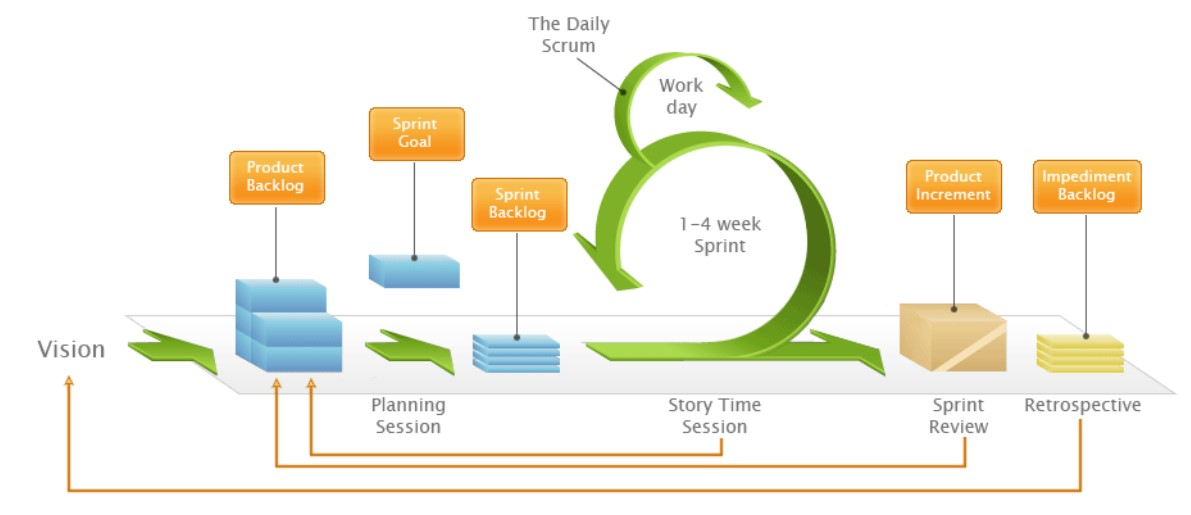
\includegraphics[width=14cm]{Images/Ciclo_Scrum.jpg}
    \caption{Ciclo de desarrollo de \textit{Scrum}}
\end{figure}

\subsubsection{Roles}
Los roles presentes en \textit{Scrum} son los siguientes:
\begin{itemize}
    \item \textbf{Product Owner}: Tiene la responsabilidad de decidir qué trabajo necesita hacerse, y maximizar el valor 
    del proyecto o producto que se esté llevando a cabo. Para ello debe tener las siguientes cualidades:
    \begin{enumerate}
        \item \textit{Saber gestionar prioridades}: Es responsable de gestionar los presupuestos, de contratar al equipo de 
        desarrollo y de explicar cuál es el valor que produce el producto en el que está invirtiendo.
        \item \textit{Toma de decisiones}: Debe ser capaz de tomar decisiones por su cuenta.
        \item \textit{Intraemprendedor}: Tiene que poder medir el valor generado y utilizar la flexibilidad de entregar cada 
        \textit{sprint} para incrementar ese valor.
    \end{enumerate}
    
    \item \textbf{Scrum Master}:Persona que ayuda al equipo y a la organización a optimizar el uso de la 
    metodología. Traslada la visión del proyecto al equipo, y elimina los obstáculos que impiden que el equipo alcance el 
    objetivo del sprint.

    \item \textbf{Development Team}: Grupo de profesionales con los conocimientos técnicos necesarios y que desarrollan el proyecto de manera
    conjunta llevando a cabo los requisitos a los que se comprometen al inicio de cada \textit{sprint}.
\end{itemize}

\begin{figure}[H]
    \centering
    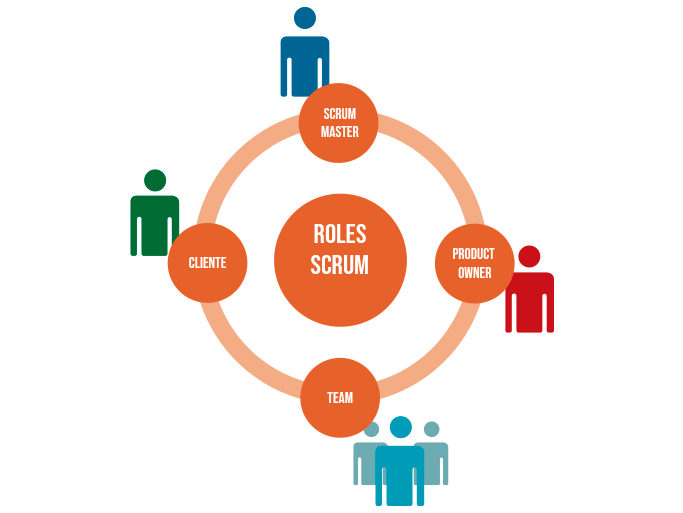
\includegraphics[width=10cm]{Images/roles.png}
    \caption{Roles en \textit{Scrum}}
\end{figure}































\section{Estructuración del documento}
El documento que se presenta está estructurado en una colección de capítulos, 
en los que se describen de manera precisa y detallada todas y cada una de 
las etapas por las que ha pasado el proyecto, desde su inicio hasta su 
conclusión. A continuación se muestra un breve resumen de los contenidos 
de cada capítulo:

\begin{itemize}
    \item \textbf{\emph{Capítulo 1. Introducción}}. El capítulo inicial 
    consiste en una introducción al proyecto, explicando los antecedentes 
    a su desarrollo, así como la motivación para ponerlo en práctica, los 
    objetivos que debe cumplir y un glosario de términos para facilitar 
    la comprensión del presente documento.

    \item \textbf{\emph{Capítulo 2. Conceptos básicos}}. Tras la introducción,
    se abordan los fundamentos necesarios para simplificar la lectura de 
    este documento. A su vez, se exponen las diferentes tecnologías de las 
    que se han aplicado para la consecución y puesta en marcha de este 
    proyecto.

    \item \textbf{\emph{Capítulo 3. Planificación del proyecto}}. Este 
    capítulo engloba toda la información relevante a aspectos de 
    suma importancia tales como la evaluación de riesgos o la planificación 
    temporal del proyecto.

    \item \textbf{\emph{Capítulo 4-\@8. Análisis, Diseño, Codificación y 
    Pruebas}}. Este conjunto de capítulos profundizan en los diversos 
    aspectos y fases que comprenden el desarrollo de un producto haciendo 
    uso de una \emph{metodología ágil}. Esto posibilita analizar y 
    enriquecer el producto en su desarrollo, mejorando así el resultado 
    final.

    \item \textbf{\emph{Capítulo 9. Manual de Instalación}}. Aquí se 
    ha desarrollado un documento con las instrucciones necesarias 
    para realizar la instalación de la aplicación.

    \item \textbf{\emph{Capítulo 10. Manual de Usuario}}. Se ha redactado 
    un manual de usuario para la aplicación, cuyo objetivo es garantizar un 
    uso eficiente y responsable de la misma por parte de los usuarios. 
    
    \item \textbf{\emph{Capítulo 11. Conclusiones}}. El último capítulo es 
    un breve repaso sobre el desarrollo del proyecto, que incluye una 
    opinión personal y un apartado de posibles mejoras que se podrían 
    realizar al proyecto en un futuro.

    % Incluir Apéndices

\end{itemize}

%\lorem{} % To do 







